\chapter{Epistemic Methods}\label{uq:epist}


This chapter covers theoretical aspects of methods for propagating
epistemic uncertainty.

\section{Dempster-Shafer theory of evidence (DSTE)} \label{sec:epist_uq:dste}

In Dempster-Shafer theory, the event space is defined by a triple 
$(\mathcal{S},\mathbb{S},m)$ which defines $\mathcal{S}$ the universal set, 
$\mathbb{S}$ a countable collection of subsets of $\mathcal{S}$, and a 
notional measure $m$. $\mathcal{S}$ and $ \mathbb{S}$ have a similar meaning 
to that in classical probability theory; the main difference is that 
$\mathbb{S}$, also known as the focal elements, does not have to be a 
$\sigma$-algebra over $\mathcal{S}$. The operator $m$ is defined to be%
%
\begin{eqnarray}
m(\mathcal{U}) 
&=&  \left\{
\begin{array}{rr}
> 0 & \mathrm{if} \ \mathcal{U} \in \mathbb{S}\\
0 & \mathrm{if} \ \mathcal{U} \subset \mathcal{S} \ \mathrm{and} \ \mathcal{U} \notin \mathbb{S} 
\end{array} \right.
\end{eqnarray}%
\begin{eqnarray}
\displaystyle\sum_{\mathcal{U} \in \mathbb{S}} m(\mathcal{U}) &=& 1
\end{eqnarray}%
%
where $m(\mathcal{U})$ is known as the basic probability assignment (BPA) of 
the set $\mathcal{U}$. In the DSTE framework, belief and plausibility are 
defined as: 

\begin{eqnarray}
	\mathrm{Bel}(\mathcal{E}) &=& \displaystyle\sum_{\{ \mathcal{U} \ | \ \mathcal{U} \subset \mathcal{E}, \ \mathcal{U} \in \mathbb{S}\}} m(\mathcal{U}) \label{eq:bel}\\
	\mathrm{Pl}(\mathcal{E}) &=& \displaystyle\sum_{\{ \mathcal{U} \ | \ \mathcal{U} \cap \mathcal{E} \neq \emptyset, \ \mathcal{U} \in \mathbb{S}\}} m(\mathcal{U}) \label{eq:pl}
\end{eqnarray}%
%
The belief Bel($\mathcal{E}$) is interpreted to be the minimum likelihood 
that is associated with the event $\mathcal{E}$. Similarly, the plausibility 
Pl($\mathcal{E}$) is the maximum amount of likelihood that could be 
associated with $\mathcal{E}$. This particular structure allows us to handle 
unconventional inputs, such as conflicting pieces of evidence (e.g. 
dissenting expert opinions), that would be otherwise discarded in an interval 
analysis or probabilistic framework. The ability to make use of this 
information results in a commensurately more informed output.  

% Appears already in Users Manual:
%Figure~\ref{fig:bel_plaus} shows example cumulative 
%belief and plausibility functions (CBF and CPF) and complementary 
%cumulative belief and plausibility functions (CCBF and CCPF, respectively). 
%This figure was taken from~\cite{helton_2004}.
%\begin{figure}[h!]% order of placement preference: here, top, bottom
% \begin{center}
% 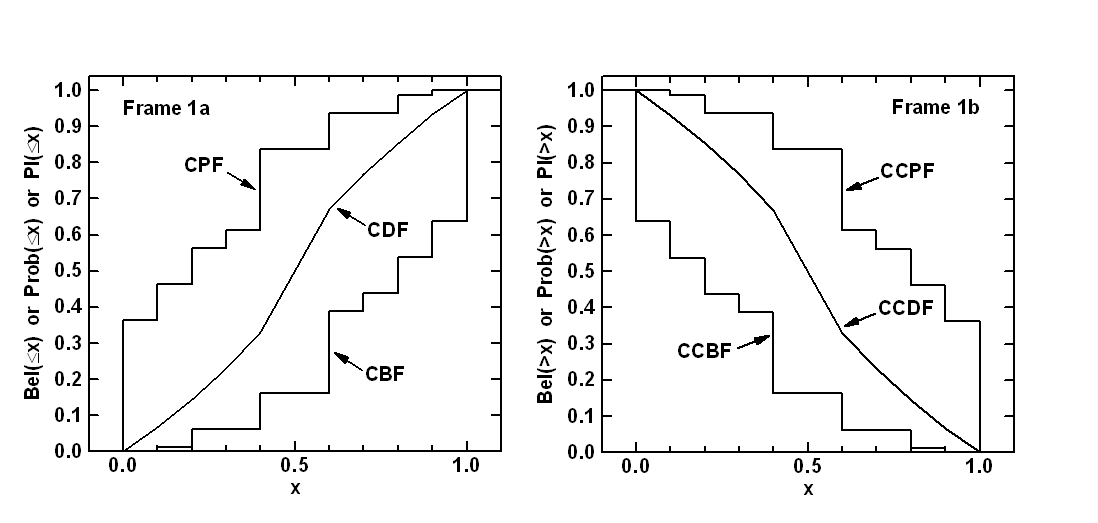
\includegraphics[width = 5in]{belief_plaus.eps}
% \caption{Example Cumulative and Complementary Cumulative Distributions for Belief and Plausibility}
% \label{fig:bel_plaus}
% \end{center} 
%\end{figure}

The procedure to compute belief structures involves four major steps:
\begin{enumerate}
  \setlength{\itemsep}{1pt}
  \setlength{\parskip}{0pt}
  \setlength{\parsep}{0pt}
\item Determine the set of $d$-dimensional hypercubes that have a nonzero 
evidential measure 
\item Compute the composite evidential measure (BPA) of each hypercube 
\item Propagate each hypercube through the model and obtain the response 
bounds within each hypercube
\item Aggregate the minimum and maximum values of the response per hypercube 
with the BPAs to obtain cumulative belief and plausibility functions 
on the response (e.g. calculate a belief structure on the response). 
\end{enumerate}

The first step involves identifying combinations of focal elements
defined on the inputs that define a hypercube. The second step
involves defining an aggregate BPA for that hypercube, which is the
product of the BPAs of the individual focal elements defining the
hypercube.  The third step involves finding the maximum and minimum
values of the response value in each hypercube, and this part can be
very computationally expensive.  Finally, the results over all
hypercubes are aggregated to form belief structures on the response.
